\documentclass[10pt]{article}
\usepackage{icmlko}

\icmlmeta{IP 파운데이션 월드모델}{968}{통제라 부른 것이 채움값이었다}{앞 두 노트가 「통제」라고 적은 열을 세어 봤다 --- 12 도메인 중 7 에서 그 열은 한 행도 안 쟀고, 거기 있던 상수 0.5 는 결측을 메우는 값이었다}

\begin{document}

\twocolumn[
\icmlheader

\begin{abstract}
앞 두 노트(966·967)는 \emph{「집단 관심의 기억은 90일보다 길다」}는 명제를 내면서
열 도메인 전부에 \textbf{「통제: \texttt{wiki\_level}, \texttt{recent\_term}」}이라
적었다. \textbf{그 문장을 정정한다.} 잰 열 개 도메인 중 \textbf{다섯}에서
\texttt{wiki\_level} 의 값 가짓수는 \textbf{1} 이고, 회귀에서 그 열을 빼도 결과가
$|\Delta\rho| \le 5.6\times10^{-17}$ 만 움직인다 --- 값이 변하는 다섯 도메인에서는
$3.5\times10^{-3} \sim 1.3\times10^{-2}$ 이니 \textbf{14 자릿수로 갈라진다}.
\textbf{상수 열을 회귀에서 빼는 것은 절편을 두 번 넣는 것이고, 그것을 「통제」라고
적는 것은 거짓 기술이다.} 그런데 더 나쁜 것이 있다 --- \textbf{그 상수는 상수가
아니었다}. 판의 자료는 $(A, M)$ 쌍이고 $M$ 은 「이 행에서 그 축을 쟀나」인데,
\texttt{wiki\_level} 은 \textbf{12 도메인 중 7 에서 $M$ 이 한 행도 안 선다}.
그 자리의 $A$ 값 $0.5$ 는 \texttt{lab/forms.py} 가
\texttt{np.where(M>0, A, 0.5)} 로 넣는 \textbf{채움값}이다. \textbf{966·967 은
$M$ 을 한 번도 안 읽었다} --- 결측 표지를 자료로 읽고 「통제」라 부른 것이다
(조항 59: 「0 행」과 「결측」은 둘이다). 세 번째로, 967 이 신고한
\textbf{Holm$(\alpha{=}.05)$ 통과 3} 은 \textbf{씨앗에 딸려 있다}. 같은 자료 ·
같은 규격 · 같은 뽑기 수(2{,}000)에서 순열 씨앗만 바꾸면 세 번째 도메인(게임)의
$p$ 가 $0.0060 \to \mathbf{0.0090}$ 이 되고 Holm 문턱 $0.00625$ 를 못 넘어
\textbf{통과가 2} 가 된다. $\hat p$ 의 몬테카를로 SE 가 $\approx 0.0019$ 라
\textbf{결정이 잡음 안에 산다}. \textbf{그래도 명제는 산다} --- 세계애니
$+0.1748$ 과 애니 $+0.1912$ 는 어느 씨앗에서도 통과하고, 두 통제를 어느 하나만
써도 부호가 안 뒤집힌다. \textbf{좁아진 것은 넓이(3\,$\to$\,2)이지 명제가 아니다.}
\end{abstract}
]

\section{무엇을 정정하는가}

\claimx{967 이 열 도메인 전부에 적은 「통제: \texttt{wiki\_level}」은 다섯 도메인에서
거짓 기술이다 --- 그 열의 값 가짓수가 1 이고, 빼도 결과가 $10^{-17}$ 만 움직인다}

규격 D 에서 잰 열 도메인의 \texttt{wiki\_level} 값 가짓수를 세면
\textbf{도서 1 · 시장팝업 1 · 애니 1 · 웹툰 1 · 팝업 1} 이고
\textbf{게임 115 · 만화 22 · 모바일 102 · 세계애니 937 · 아이돌 28} 이다.
가짓수가 1 인 다섯에서 그 열을 통제에서 빼면 $\rho$ 가 정확히 그대로다
(그림~\ref{fig:dead} 오른쪽). 그중 \textbf{팝업은 $\Delta = 0.0$ 이 부동소수로도
정확}하고, 나머지 넷은 $|\Delta| \le 5.6\times10^{-17}$ 이다.

\textbf{「바이트 동일」은 구현에 딸린 성질이다.} 967 과 그 비평자는
\texttt{lstsq} 를 써서 정확히 $0$ 을 봤고, 이 노트는 \texttt{pinv} 사영을 써서
$10^{-17}$ 이 남는다. \textbf{실질은 같다} --- 어떤 눈금에서도 $10^{-17}$ 은 뜻이
없다. 갈라지는 것은 「인자를 바꿔도 출력이 안 변한다」는 사실 쪽이지 그 자릿수가 아니다.

\claimx{그 상수는 상수가 아니라 채움값이다 --- \texttt{wiki\_level} 은 12 도메인 중
7 에서 마스크가 한 행도 안 서고, 966·967 은 마스크를 한 번도 안 읽었다}

이 저장소의 판은 도메인마다 $(A, M, y, t)$ 를 들고 있고 $M[i,j]$ 는
\textbf{「$i$ 행에서 $j$ 축을 쟀나」}다. 축이 그 도메인에 안 붙으면 $M$ 은 전 행 $0$ 이고
$A$ 는 그 자리에 \textbf{0.5} 를 들고 있다 --- \texttt{lab/forms.py} 가 모형에
넘기기 전에 \texttt{np.where(M[:,j]>0, A[:,j], 0.5)} 로 채우는 그 값이다.

\texttt{wiki\_level} 의 마스크가 한 행도 안 서는 도메인은 \textbf{일곱}이다 ---
도서 · 시장팝업 · 애니 · 영화 · 웹툰 · 팝업 · 펀딩(그림~\ref{fig:dead} 왼쪽).
966·967 은 \texttt{A[:, nm.index("wiki\_level")]} 만 읽었고 $M$ 을 안 읽었다.
\textbf{결측 표지를 자료로 읽었고, 그것을 「통제」라 불렀다.}

이 구별은 값 하나를 바꾸는 것이 아니라 \textbf{문장의 종류를 바꾼다}. 「이 도메인에서는
수준을 통제해도 효과가 남는다」와 「이 도메인에서는 수준을 아예 안 쟀다」는 다른 주장이다.

\begin{figure}[t]
\centering
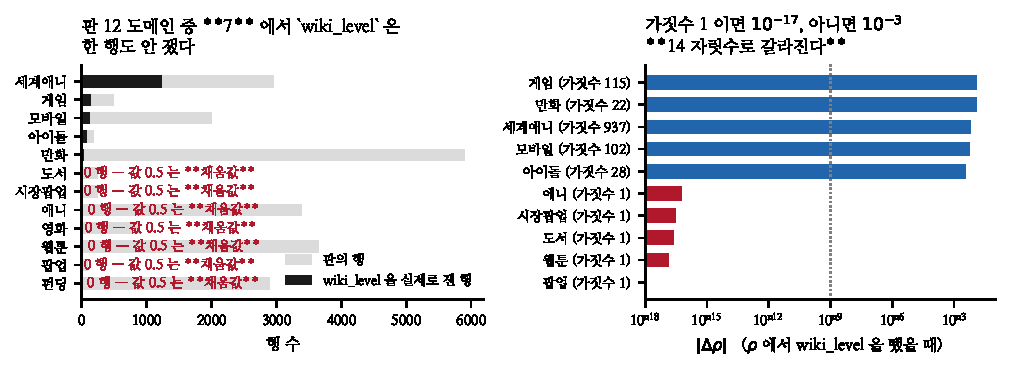
\includegraphics[width=\columnwidth]{figs/deadcontrol.pdf}
\caption{\textbf{왼쪽}: 도메인별 판의 행 수(회색)와 \texttt{wiki\_level} 을 실제로 잰
행 수(검정). 일곱 도메인에서 후자가 $0$ 이다. \textbf{오른쪽}: 규격 D 에서
\texttt{wiki\_level} 을 통제에서 뺐을 때 $|\Delta\rho|$(로그 눈금). 가짓수 1 인
도메인(붉음)과 아닌 도메인(회색)이 14 자릿수로 갈라진다.}
\label{fig:dead}
\end{figure}

\claimx{967 의 「Holm 통과 3」은 씨앗에 딸려 있다 --- 같은 자료·같은 규격에서 순열
씨앗만 바꾸면 통과가 2 다}

967 은 세계애니 $+0.1747$ · 애니 $+0.1912$ · 게임 $+0.2311$ 셋이 Holm$(\alpha{=}.05)$
을 통과했다고 적었다. 이 노트가 \textbf{다른 구현·다른 씨앗}으로 같은 규격을 다시 재면
$\rho$ 는 소수 넷째 자리까지 재현되는데(세계애니 $+0.1748$ · 애니 $+0.1912$ ·
게임 $+0.2311$) \textbf{게임의 $p$ 가 $0.0060$ 에서 $0.0090$ 으로 움직인다}.
Holm 문턱은 $0.05/8 = 0.00625$ 이고, $\hat p$ 는 뽑기 $2{,}000$ 의 이항 추정이라
$\mathrm{SE} \approx \sqrt{p(1-p)/2000} \approx 0.0019$ 다.
\textbf{$|p - \text{문턱}|$ 이 1 SE 안이다} --- 통과/탈락이 동전 던지기다.

그러므로 \textbf{순열 $p$ 로 다중비교 문턱을 넘었다고 말할 때는 몬테카를로 SE 를
병기해야 한다}. 이것을 상시 조항으로 올렸다(조항 65-⑤).

\section{그래도 명제는 산다}

세계애니($n{=}1{,}075$)와 애니($n{=}362$)는 어느 씨앗에서도 Holm 을 통과한다
($p \le 0.001$). 그리고 세계애니의 효과는 \textbf{순수한 조건부 효과}다 ---
생 $\rho$ 가 $-0.0078$ 인데 두 통제를 뺀 뒤 $+0.1748$ 이다. 매개 인공물은 아니다:
\texttt{excite} $=$ \texttt{recent} $-$ \texttt{long} 이라 \texttt{recent} 는 하류
매개가 아니라 \texttt{excite} 의 \textbf{성분}이고, 어느 통제 \textbf{하나만} 써도
부호가 안 뒤집힌다(\texttt{level} 만 $+0.1642$ · \texttt{recent} 만 $+0.1684$).

\textbf{다만 추정치가 얇은 잔차 공간에 산다.} 세계애니에서 두 통제의 순위 상관은
$+0.9194$ 이고, \texttt{level} 을 뺀 뒤 \texttt{recent} 에 남는 분산은
\textbf{15.5\%} 다. 아이돌은 더 심해서 상관 $+0.9742$ · 남는 분산 \textbf{5.1\%} 이고
$n{=}30$ 이다. \textbf{이 표본들은 두 통제를 원리상 못 가른다} --- 「효과가 가짜다」가
아니라 「이 자료로는 그 질문에 답할 수 없다」이다.

\section{한 문장}

\textbf{통제가 살아 있는지 세지 않고 조건부 효과를 해석하면, 무엇을 통제했는지 모르는 채
해석하는 것이다.} 이 노트가 한 일은 새 자료를 대는 것이 아니라 \textbf{이미 있던 열의
가짓수를 세는 것}이었고, 그 셈 하나로 앞 두 노트의 방법 문장 하나가 거짓으로 드러났다.
\textbf{세는 데 든 것은 코드 스무 줄이다.}

\end{document}
